\documentclass[letterpaper]{jpconf}

\usepackage{graphicx}

\usepackage{hyperref}

\usepackage{cite}

\newcommand{\maestro}{{\sffamily Maestro}}
\newcommand{\castro}{{\sffamily Castro}}
\newcommand{\starkiller}{{\sffamily StarKiller}}
\newcommand{\nyx}{{\sffamily Nyx}}
\newcommand{\amrex}{{\sffamily AMReX}}


\begin{document}

\title{Meeting the Challenges of Modeling Astrophysical Thermonuclear Explosions:
\castro, \maestro, and the \amrex\ Astrophysics Suite}

\author{M. Zingale$^1$,
        A.~S. Almgren$^2$,
        M.~G. Barrios Sazo$^1$,
        V.~E. Beckner$^2$,
        J.~B. Bell$^2$,
        B. Friesen$^2$,
        A.~M. Jacobs$^3$,
        M.~P. Katz$^4$,
        C.~M. Malone$^5$,
        A.~J. Nonaka$^2$,
        D. Willcox$^1$, and
        W. Zhang$^2$}

\address{$^1$Department of Physics and Astronomy, Stony Brook
  University, Stony Brook, NY 11794-3800 USA}

\address{$^2$Center for Computational Sciences and Engineering,
  Lawrence Berkeley National Lab, Berkeley, CA 94720 USA}

\address{$^3$Department of Physics and Astronomy, Michigan State
  University, East Lansing, Michigan 48824 USA}

\address{$^4$Nvidia Corporation}

\address{$^5$Los Alamos National Laboratory, Los Alamos, NM, 87545 USA}

\begin{abstract}
We describe the \amrex\ suite of astrophysics codes and their
application to modeling problems in stellar astrophysics.
\maestro\ is tuned to efficiently model subsonic convective flows
while \castro\ models the highly compressible flows associated with
stellar explosions.  Both are built on the block-structured adaptive
mesh refinement library \amrex.  Together, these codes enable a
thorough investigation of stellar phenomena, including Type Ia
supernovae and X-ray bursts.  We describe these science applications
and the approach we are taking to make these codes performant on
current and future many-core and GPU-based architectures.
\end{abstract}




\section{Introduction}

Astrophysical explosions come in many flavors: gravitational and
thermonuclear supernovae, unstable burning on the surface of compact
objects, and explosive ignition of burning stages in stellar
evolution.  Accurate modeling of these events requires the coupling of
hydrodynamics, gravity, thermonuclear reactions, and in some cases,
radiation and magnetic fields.  Further, these environments are
characterized by a wide range of lengthscales, from the size of the
star or binary system down to the burning zone width and dissipation
scales.  Temporal scales are equally impressive---stellar evolution
occurs over 10s of millions to billions of years, the simmering phase
leading up to explosions lasts millenia to days or hours, and the
explosion can be over in seconds to hours.  The radiation leakage,
which leads to the observables we see lasts from hours to months.

No single algorithm meets all of the demands imposed by these events.
Instead, we advance our understanding of these events by piecing
together simulations of different phases of the evolution from
different codes.  Here we discuss our simulation codes, \maestro\ and
\castro\ designed to perform three-dimensional models of the early
subsonic evolution leading to runaway and the subsequent expolosion.
Together this suite of codes allows us to address many problems in
stellar and nuclear astrophysics.  We describe some of the design
details, the current architecture of the code, and some applications
below.

\section{Science drivers and challenges}

Our interests are thermonuclear explosions, including Type Ia
supernovae, X-ray bursts, and novae.  The basic ingredients for these
events are thermonuclear energy release and a degenerate equation of
state that allows a runaway to build without a pressure response.
Most of the current models for these events are characterized by a
long timescale ``simmmering'' phase where reactions heat the star or
layer and drive convection.  Eventually, reactions become vigorous
enough that a runaway takes place, perhaps with an accompanying
burning front that spreads through the star.

\subsection{Type Ia supernovae}

The largest open theoretical question for SNe Ia is---what is the
nature of the progenitor?  About 20 years ago, the community had
mostly converged up the single-degenerate scenario---a
Chandrasekhar-mass C/O white dwarf that accretes from its companion,
eventually leading to runaway at the center that burns through the
star (see~\cite{hillebrandtniemeyer2000} for the state of the field
at that time).  Since then, the wealth of observations has show that
there is a lot of diversity in SNe Ia, and searches for progenitor
systems have not shown that Chandra-mass white dwarfs can explain all
SNe Ia.  Today, merging white dwarfs (the double degenerate scenario)
have become the most popular model.  Other progenitors, like He
burning on the surface of a sub-Chandra white dwarf have also seen
interest in explaining some of the observed diversity.

There are open questions in all of these scenarios which can be
addressed through simulation.  For the Chandra and sub-Chandra models,
what is the distribution (spatial and temporal) of the hotspots setup
by turbulent convection that give rise to burning fronts.  Can you
create a detonation in the He layer in the double detonation model?
For double degenerates, does the burning take place promptly?  Is it
possible to accurate model a detonation in this case, given our
resolution constraints?  These are some of the questions we seek to
answer.

\subsection{XRBs}

X-ray bursts, the burning of accreted H/He on the surface of a neutron
star, can be important probes of neutron star structure.  Interpreting
observations requests that we understand what we are seeing, which can
be influenced by the products of the burning and how the burning
spreads across the star.  Many efforts have focused on different
aspects of these events.  One-dimensional models capture the
energetics well and inform us about the nucleosynthesis
\cite{woosley-xrb}.  Global models show the importance of rotation in
confining the burning \cite{SPIT_ETAL02}, why models inspired from
atmospheric science can explore the vertical structure
\cite{cavecchi:2012}.  However, the resolution differences from the
scale of the burning to a reasonable fraction of the neutron star
surface has prevented detailed explorations of the burning in resolved
calculations and how it feeds back on the flame structure and
propagation.  


\subsection{Requirements}

conservation of gravity / angular momentum
                strong coupling of hydrodynamics and burning
                long timescale evolution

                3-d, turbulence, instabilities, rotation, ...

\section{AMReX Astrophysics Suite}

Our suite of application codes is built on the
\amrex\ block-structured adaptive mesh refinement (AMR) library.  The
basic programming model is that \amrex\ manages the grid
data-structures and parallelism, and calls the computational kernels
on a patch-by-patch basis.  AMReX supports subcycling in time, which
we use in \castro.

\amrex\ uses a hybrid approach to parallelism.  Tiling is used to
logically subdivide AMR patches to increase the parallelism for
OpenMP, without incurring the memory overheads that using many more
smaller grids would bring~\cite{tiling}.  This strategy is especially
important for many core architectures like the Intel Phi.  Ongoing development
is being done to support GPU offloading, using managed memory provided
by the latest generations of GPUs.

There are many application codes built on \amrex, including those in
combustion, ...  In astrophysics, these include \maestro\ and
\castro\ for stellar and nuclear astrophysics applications and
\nyx~\cite{nyx} for cosmological applications.  Here we focus on the
former two.

\subsection{\maestro}

\maestro~\cite{MAESTRO:Multilevel} is a low Mach number stellar
hydrodynamics code.  \maestro\ has been applied to convection in the
Chandrasekhar-mass model for Type Ia supernovae (SNe Ia)
\cite{ZABNW:IV,wdconvect,wdturb}, the sub-Chandra model for SNe Ia
\cite{subchandra,subchandra2} X-ray bursts~\cite{xrb,xrb2,xrb3}, and
convection in massive stars \cite{ms_cc}.

\maestro\ decomposes the state into a one-dimensional hydrostatic base
state and a three-dimensional Cartesian state that evolves the
departures from HSE.  A constraint equation is derived by requiring
that the pressure everywhere be close to the background hydrostatic
state.  The constraint acts to enforce instantaneous acoustic
equilibriation, effectively filtering soundwaves from the system,
while retaining the compressibility effects due to the background
stratification of the star and local heat release, as well as the
hydrostatic adjustment of the star.  In this fashion, it is more
general than traditional anelastic methods.  Low speed methods have
seen a lot of recent development~\cite{kleinpauluis,vasil:2013}, which
has been incorporated into \maestro.  The next development effort for
\maestro\ will be to allow for moderate rotation of the star.

\subsection{\castro}

\castro~\cite{castro,castroII,castroIII} is a fully-compressible
radiation hydrodynamics code that supports arbitrary equations of
state, nuclear reaction networks, and Poisson gravity.  \castro\ has
been applied to core-collapse supernovae~\cite{castro-ccsne},
population III pair-instability
supernovae~\cite{castro-pairinstability}, and white dwarf mergers as a
model for SNe Ia~\cite{wdmergerI}.  Recent work has focused on
improving energy conservation with gravitational and rotational
sources and new integration methods that more accurately couple hydro
and reactions.

For \maestro\ simulations that evolve from the subsonic regime to the
sonic regime, we have demonstrated the ability to restart the
calculations in \castro\ to continue the evolution into the sonic
regime~\cite{scidac-petascale,malone:2014} (in this case, for Chandra
model SNe Ia).

\subsection{\starkiller\ Microphysics}

\maestro\ and \castro\ share the same microphysics, available as the
\starkiller\ astrophysics github
project\footnote{\url{https://github.com/StarKiller-astro/microphysics/}}.
This includes equations of state and nuclear reaction networks.  The
reaction networks are written such that that rates and integration
strategy are decoupled, allowing us to change the integration strategy
for a set of rates.  


\subsection{Open source and reproducibility}

All of our simulation codes are open source and follow a fully open
development model---the development git repos are hosted on
github\footnote{\url{https://github.com/AMReX-Astro/}}, available for
anyone to see and contribute to using issues and pull-requests.
{\em All source files, model files, input parameters, etc.\ for any
published science results are also available in the code repos.}  When
feasible, the git hashes for the published results are included in paper
acknowledgements.


\section{Parallel Performance and GPUs}


GPUs

     . show Don's plot

\begin{figure}[t]
\centering
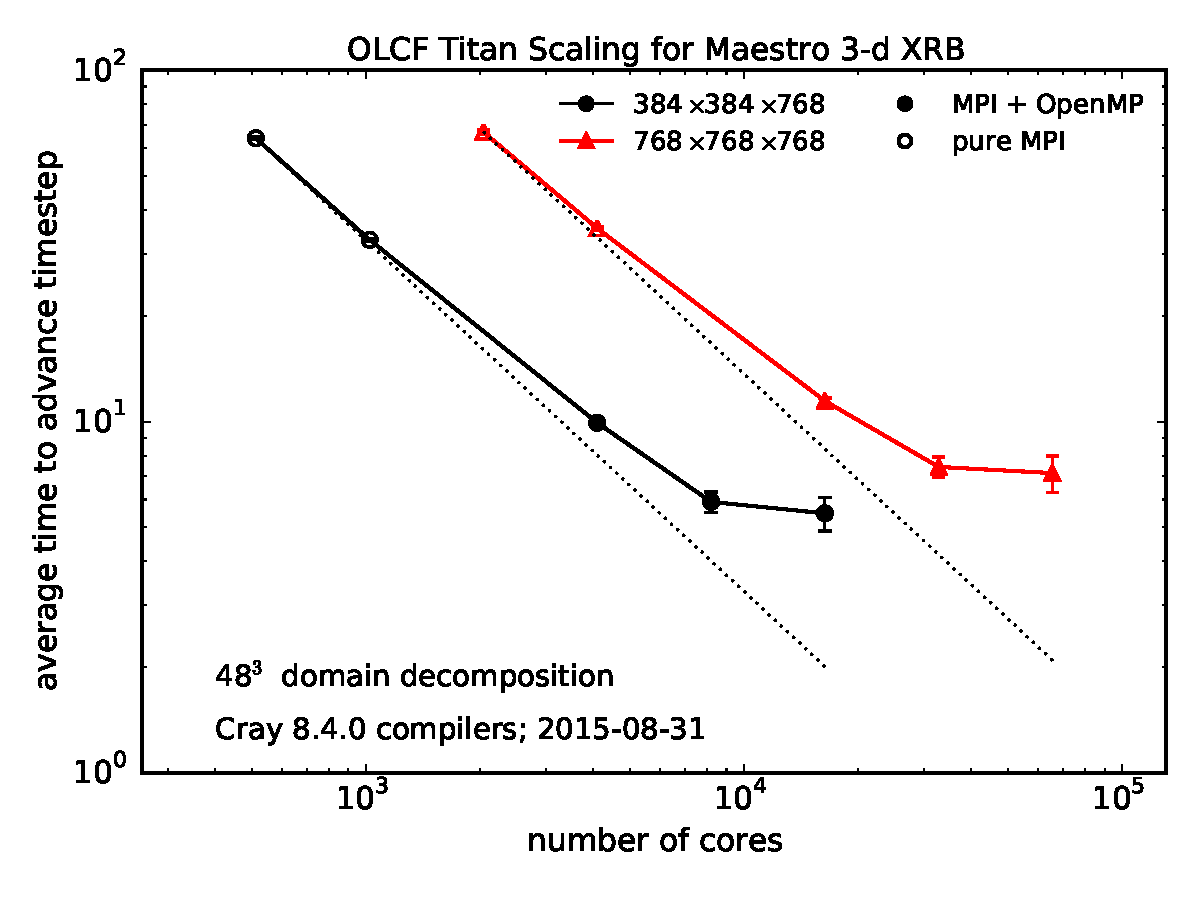
\includegraphics[width=0.5\linewidth]{titan_xrb_scaling}
\caption{\label{fig:maestro_scaling} blah}
\end{figure}

Figure~\ref{fig:maestro_scaling} shows strong scaling for \maestro\ on the 3-d
XRB problem.

show new scaling

Our latest focus has been on GPUs



\section{Science results}

\begin{figure}[t]
\centering
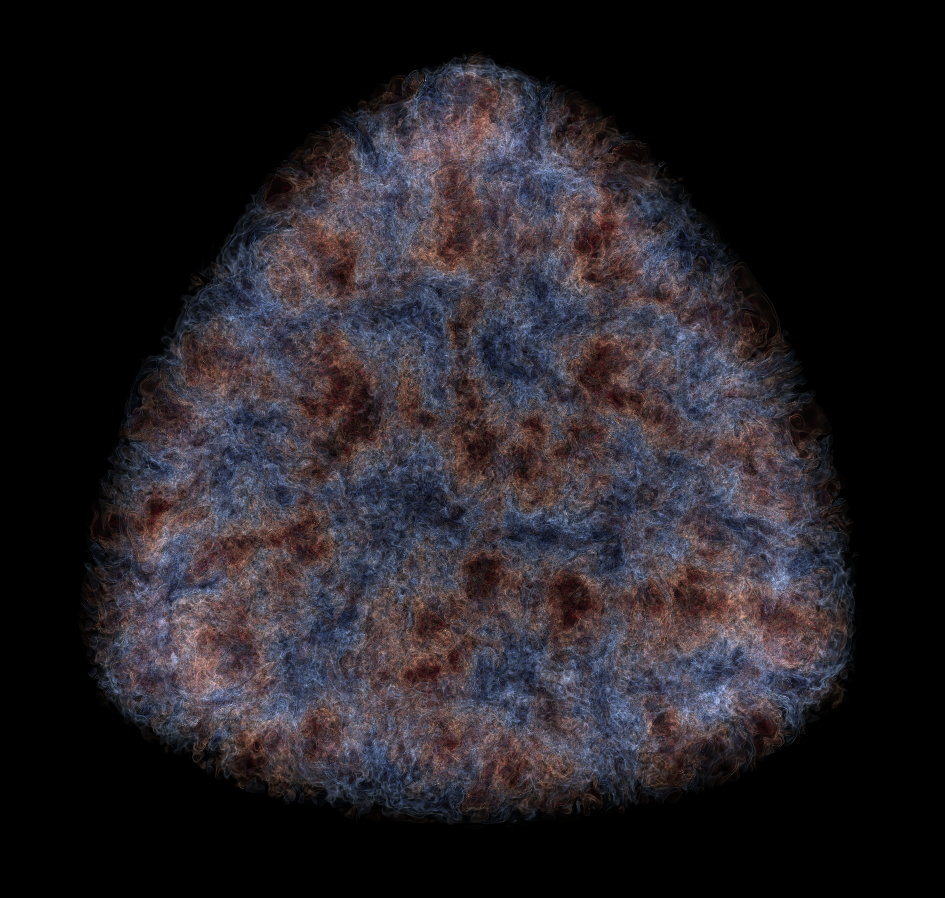
\includegraphics[height=1.8in]{subch_h}
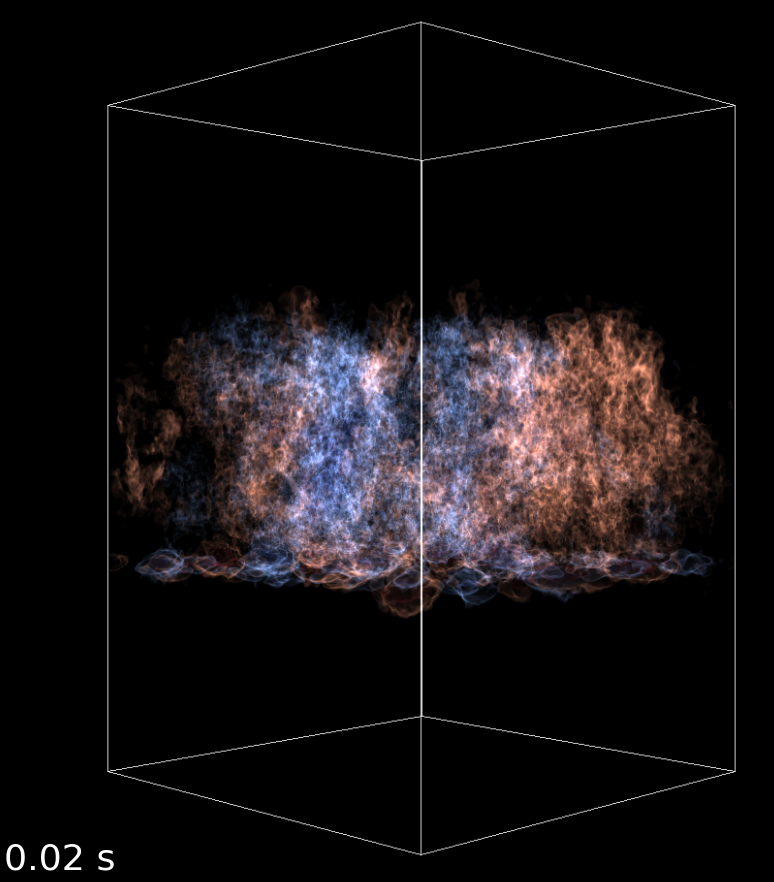
\includegraphics[height=1.8in]{xrb_compact}
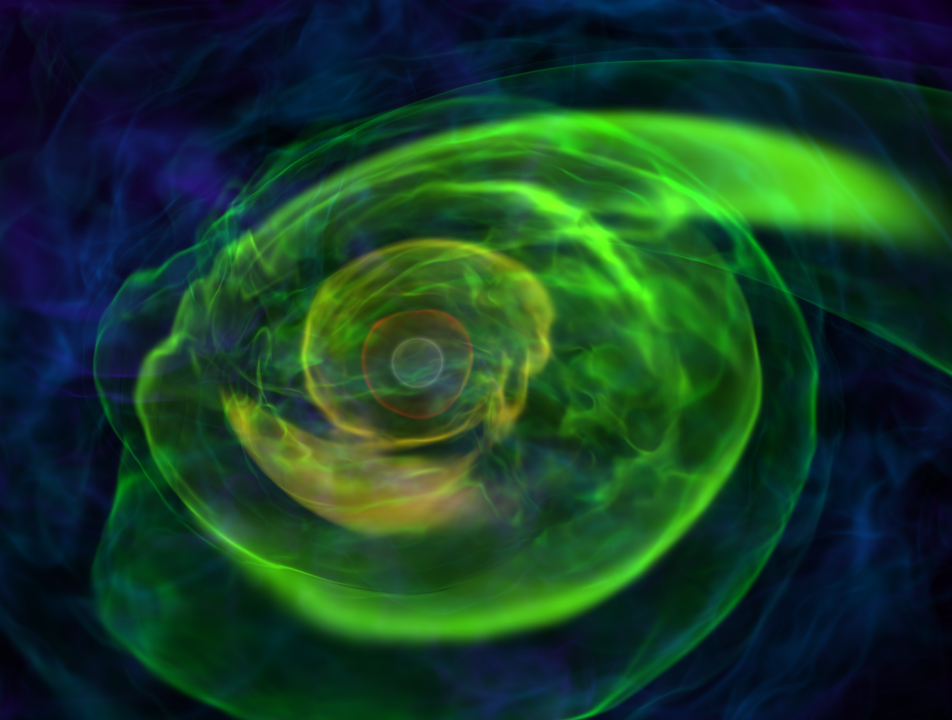
\includegraphics[height=1.8in]{wdmerger_08030_new}
\caption{\label{fig:current-runs} (left) Convective plumes in a
  \maestro\ sub-Ch calculation. (center) Vertical velocity showing the
  convective structure in a \maestro\ XRB calculation. (right)
  Snapshot of a \castro\ simulation of the merger of two white dwarfs,
  with 0.90 and 0.81 solar masses. The contours represent density
  levels.}
\end{figure}

Figure~\ref{fig:current-runs} shows some of our most recent science simulations.

\ack The work at Stony Brook was supported by DOE/Office of Nuclear
Physics grant DE-FG02-87ER40317 and NSF award AST-1211563.  An award
of computer time was provided by the Innovative and Novel
Computational Impact on Theory and Experiment (INCITE) program.  This
research used resources of the Oak Ridge Leadership Computing Facility
at the Oak Ridge National Laboratory, which is supported by the Office
of Science of the U.S. Department of Energy under Contract
No.\ DE-AC05-00OR22725.  This research used resources of the National
Energy Research Scientific Computing Center, which is supported by the
Office of Science of the U.S. Department of Energy under Contract
No.\ DE-AC02-05CH11231.  Results in this paper were obtained using the
high-performance LIred computing system at the Institute for Advanced
Computational Science at Stony Brook University, which was obtained
through the Empire State Development grant NYS \#28451.  The GPU work
benefited from a grant of an Titan X Pascal board from Nvidia Corp
through the GPU Grant Program.
                          

\section*{References}

\bibliographystyle{iopart-num}
\bibliography{ws}


\end{document}
